\section{General Overview of a Single Simulation}
\label{sec:general-overview-of-simulation-output}
First, let us describe the outcome of the simulation framework which is visualized in the Figure~\ref{fig:single-simulation-example}.
The simulation framework provides this graph for each possible simulation.

\begin{figure}
    \centering
    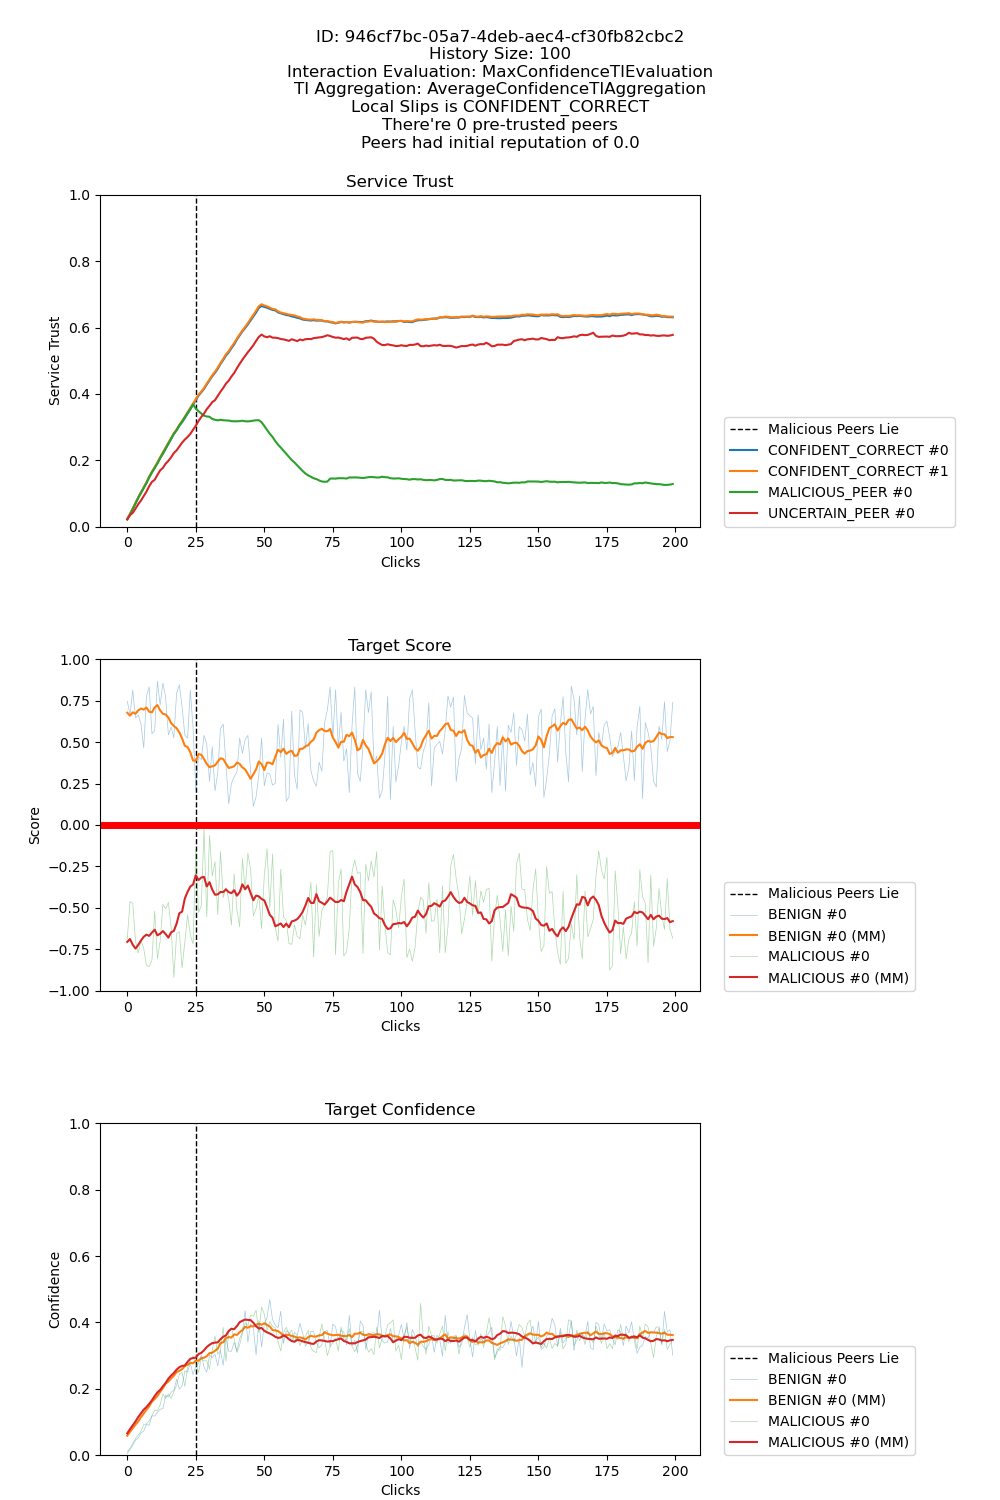
\includegraphics[width=1.0\textwidth]{assets/example_evaluation.png}
    \caption{Example of a single simulation}
    \label{fig:single-simulation-example}
\end{figure}

The graph's headline explains which setup parameters were used for the trust model. In the case of Figure~\ref{fig:single-simulation-example} Fides used interaction evaluation strategy $MaxConfidenceTIEvaluation$ (section~\ref{subsec:MaxConfidenceTIEvaluation}).
For aggregating the threat intelligence, Fides used the aggregation described in  section~\ref{sec:network-intelligence-aggregation}.
The local Slips instance behaved like confident correct peer outlined in  section~\ref{subsubsec:confident-correct-peer}.

The graph on top in Figure~\ref{fig:single-simulation-example} shows the development of the \textit{service trust} $st_{i, j}$ (section~\ref{subsec:service-trust}) on the vertical axis over \textit{time} on the horizontal axis. As mentioned in the section~\ref{sec:environment-simulation}, the time is measured in \textit{clicks}.
One can see multiple peers that were involved in the simulation and their respective behavior. All possible behaviors are described in the section~\ref{sec:peers-behavioral-patterns}.
There were four different peers that were communicating with the local instance of Fides, two of them were \textit{confident correct}, one was an \textit{uncertain peer} and the last one was a \textit{malicious peer}.

The dotted line indicates the time when the malicious peers start lying.
One can see that during this first period, when the malicious peers were not lying \textit{(before the line)}, they were gaining the service trust.
In the case of Figure~\ref{fig:single-simulation-example} this happened at click 25 when the malicious peers started lying.
After that, it is clear that they started to lose the service trust.

The second graph in Figure~\ref{fig:single-simulation-example} shows the \textit{target score} during the time (\textit{clicks}).
The target score $S^{k}_{T}$ (section~\ref{sec:network-intelligence-aggregation}) is the part of the aggregated network threat intelligence, that was computed from the scores and confidences provided by each peer.
The score was calculated by Fides at click $k$ for target $T$.

The score graph contains two different targets, one that is according to the ground truth malicious and the second, that was benign.
We also included the moving average value (indicated as MM) within the window of 10 clicks to make the graph clear.

Finally, third graph, displays the aggregated confidence $C^{k}_{T}$ (section~\ref{sec:network-intelligence-aggregation}) over time (\textit{clicks}).
The graph is similar to the score, we include raw values for each time window and target as well as the moving average within the window of 10 clicks.

In this example output graph, it can be seen that Fides was clearly able to identify that the malicious peer started to lie after click 25 because of the service trust $st^{k}_{i,j}$ for this peer that fell down almost instantly.
At the same time, we can see that on the score graph, the $S^{k}_{T}$ for both targets were skewed and started to get closer to $0$ because the malicious peer had already gained service trust and thus the threat intelligence provided by it had an impact on the final $S^{k}_{T}$.
However, after Fides figured out, that the peer is lying, it lowered its service trust for this peer and the score started to recover closer to the baseline.